% !TEX encoding = UTF-8
% !TEX TS-program = pdflatex
% !TEX root = ../tesi.tex

%**************************************************************
\chapter{Lo stage nella strategia aziendale}
\label{cap:lo stage nella strategia aziendale}
%**************************************************************

\section{Aspettative personali}
La mia esperienza lavorativa si è sempre limitata a piccoli lavori occasionali, un periodo in cui ho svolto un progetto esterno per un'azienda ed in seguito uno stage nella stessa azienda, entrambi durante la scuola secondaria di secondo grado.\\
Già da queste piccole esperienze, avevo capito quanto la pratica sul campo fosse una valida opportunità per applicare attivamente quanto studiato durante la carriera da studente e, inoltre, apprendere nuove nozioni. 
Dall'attività di stage, quindi, le mie speranze erano quelle di poter apprendere nuove nozioni e consolidare quelle già in mio possesso tramite un approccio che fosse più pratico di quello che normalmente viene utilizzato all'interno dell'ambiente universitario. \\
I miei obiettivi iniziali per un progetto di stage erano quindi i seguenti:
\begin{itemize}
	\item Entrare in contatto con nuove tecnologie;
	\item Vedere e capire il funzionamento di una realtà aziendale in ambito tecnologico ed ICT;
	\item Poter lavorare con il supporto di personale qualificato;
	\item Vedere in pratica come le nozioni apprese in aula o da studio personale vengono realmente applicate nel mondo lavorativo.
\end{itemize}
Per far sì che le mie opzioni di scelta fossero quanto più numerose possibili, ho deciso di partecipare all'iniziativa denominata Stage-IT\footcite{site:stageit} organizzata dall'Università di Padova. Prima di andare all'evento, ho stilato una lista di possibili aziende a cui presentarmi, facendo soprattutto attenzione ai progetti proposti. Durante l'evento ho quindi colto l'occasione per discutere dell'attività di stage con molteplici aziende. Molte di loro operavano in campi che a mio parere non risultavano essere particolarmente interessanti, ma qualche azienda ha colto la mia curiosità e mi ha permesso di avere con loro un colloquio di presentazione reciproca. Alcune di queste erano più interessate a stage per inserimento lavorativo e di durata di circa 6 mesi, che ad uno finalizzato per la tesi, e quindi ho dovuto scartarle a priori nonostante il mio interesse. \\
Fortunatamente, l'azienda IT Euro Consulting proponeva uno stage adeguato per lo sviluppo della tesi e gli argomenti coinvolti erano pienamente di mio interesse: durante il colloquio conoscitivo comunque, l'azienda non mi ha subito presentato un progetto di stage, ma piuttosto mi ha esposto la struttura aziendale, la focalizzazione dello stage nell'ambito \textit{big data} e la propensione dell'azienda per l'innovazione e l'interesse a conoscere nuovi punti di vista come quello di uno studente universitario. Tutto ciò mi ha attratto fin da subito e quindi, dopo un paio di incontri successivi avvenuti in azienda, l'azienda ha proceduto alla presentazione del progetto di stage vero e proprio.

Considerando i miei obiettivi e la lista di aziende con le quali ho avuto un contatto a Stage-IT, ho deciso di svolgere il progetto di IT Euro Consulting, in quanto di maggiore interesse rispetto ai progetti offerti da altre aziende.

%**************************************************************
\section{Aspettative aziendali}
Quest'anno IT Euro Consulting ha deciso, per la prima volta, di attivare un progetto di stage universitario che non avesse come fine ultimo l'assunzione del tirocinante. I motivi di questa scelta sono molteplici e condivisibili. \\
In primo luogo è necessario distinguere i percorsi che l'azienda ha deciso di far intraprendere ai diversi tirocinanti in base allo scopo dello stage. \\ 
Per gli studenti, appena laureati o laureandi, il cui fine è l'assunzione al termine del tirocinio, l'azienda ha previsto un periodo di lavoro di circa 6 mesi, durante il quale, dopo il primo periodo formativo, lo stagista viene inserito in progetti già avviati e quindi affiancati dal team a cui è assegnato il lavoro. Negli ultimi 3 anni, infatti, l'azienda ha ampliato i reparti sviluppo e \textit{big data} ed ha assunto molteplici persone in seguito ad uno stage o tirocinio. Oggigiorno infatti la maggior parte del personale appartenente ai reparti sviluppo e \textit{big data} ha un titolo di laurea in Informatica o Ingegneria. \\
Nell'altro caso, ovvero lo stage curricolare, come di mio interesse, la durata è di circa 300-350 ore e si distingue in una fase di apprendimento ed in una fase di progetto, sempre affiancati da uno o più tutor interni. Durante il progetto, il tirocinante ha maggiore libertà sulla scelta delle tecnologie che utilizzerà e su decisioni progettuali. Queste poi vengono discusse con il tutor in modo da correggere eventuali scelte errate frutto dell'inesperienza del tirocinante. \\
I vantaggi di questi due percorsi sono in parte comuni: in primo luogo si ha l'inserimento in organico di nuove risorse provenienti dal mondo universitario. Assumere anche solo provvisoriamente una figura per uno stage proveniente dal mondo universitario giova all'azienda in quanto il personale ha la possibilità di confrontarsi ed aggiornarsi con costui sui nuovi insegnamenti e corsi universitari. Questa vicinanza è però anche utile per lo studente, in quando ha la possibilità di vedere concretamente come quanto appreso in aula sia implementato effettivamente nel mondo reale e di capire come funzioni realmente un'azienda, se non ha già avuto esperienze simili durante la sua carriera.
Il secondo motivo è la possibilità per l'azienda di comprendere il livello di preparazione medio degli studenti universitari ed essere attivi nello scrutare quelli più meritevoli che possono portare ad un vantaggio competitivo considerevole.
Per quanto riguarda il mio percorso di stage, quello curricolare, si possono riconoscere altri due vantaggi ed entrambi derivano dalla maggior libertà che si concede allo studente per risolvere problemi che solitamente in azienda si risolverebbero tramite soluzioni già consolidate. La possibilità di sfruttare nuove tecnologie senza la necessità di perdita di tempo del personale aziendale, permette di rimanere aggiornati sul continuo rilascio di librerie e \textit{framework} che potrebbero portare benefici ai vari team in termini di efficienza, sia sul tempo di sviluppo del software, sia per quanto riguarda le performance del prodotto stesso.
La maggiore libertà sulla progettazione e lo sviluppo concessa allo stagista consente anche di valutare vantaggi e svantaggi di soluzioni architetturali che il personale aveva scartato prematuramente o che non aveva considerato a priori.\\
Alla fine dello stage, l'azienda si aspettava di avere una \gls{web app} che esponesse i dati precedentemente recuperati dal \gls{cluster}, esaminati ed elaborati in modo da facilitare il successivo sviluppo del modello per stimare il target desiderato.\\
Tutto ciò mi ha portato prima dell'inizio dell'attività di stage, a concordare insieme al tutor aziendale i requisiti del progetto, che durante lo stage sono rimasti fedeli al Piano di Lavoro. L'unico punto leggermente modificato riguarda infatti un disguido tecnico relativo ad un problema con il personale aziendale, il quale non ha potuto configurare l'accesso al \gls{cluster} tramite \gls{Java JDBC}.\\
Per poter gestire al meglio lo stage ed avere una buona elasticità sugli obiettivi da raggiungere, il tutor li ha suddivisi in due categorie: obiettivi obbligatori e obiettivi desiderabili.

\begin{table}[!h] %
	\caption{Obiettivi dello stage} \label{obiettivi_stage}
	\label{tab:obiettivi-stage}
	\begin{tabular}{|l|}
		\hline
		\\[-2mm]
		\textbf{Obiettivi obbligatori}\\
		\hline
		\\[-2mm]
		Caricare, estrarre e compiere semplici operazioni su file presenti nel \gls{cluster}	\\
		\hline
		\\[-2mm]
		Svolgere semplici operazioni con Hive/Impala su tabelle già esistenti, con creazione \\ di nuove tabelle contenenti statistiche riassuntive e porzioni di dati	\\
		\hline
		\\[-2mm]
		Svolgimento di una semplice analisi dati con Spark, dall'ingestion all'esame del \\ \textit{dataset}, salvando i risultati in formato tabellare CSV	\\
		\hline
		\\[-2mm]
		Sviluppo di un \gls{Web Service} RESTful in grado di presentare in formato JSON i \\ risultati CSV \\
		\hline
		\hline
		\\[-2mm]
		\textbf{Obiettivi desiderabili}\\
		\hline
		\\[-2mm]
		Creazione di nuove tabelle tramite l'utilizzo di \textit{query} SQL innestate e con \\ operazioni complesse \\
		\hline
		\\[-2mm]
		Sviluppo di una semplice applicazione capace di interfacciarsi con i dati prodotti \\ da Spark e riassumere graficamente i risultati \\
		\hline
		\\[-2mm]
		Sviluppo di un'applicazione Java EE \textit{3-tier}, composta da un'interfaccia grafica \\ HTML5/Angular in grado di visualizzare i dati dei risultati in modalità grafica e \\ un Web Service RESTful per la presentazione dei dati in formato JSON recuperati \\ con Hive/Impala \\
		\hline
	\end{tabular}
\end{table}%
\clearpage
\begin{figure}[!h] 
	\centering 
	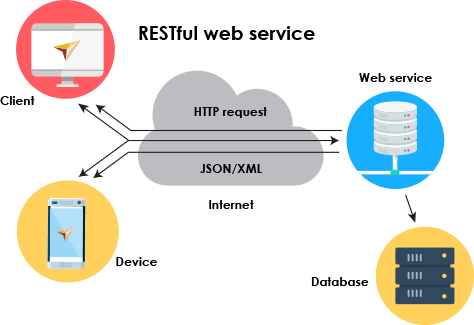
\includegraphics[width=0.75\columnwidth]{web-service}
	\caption{RESTful Web Service (Fonte: \href{https://goo.gl/zvrBJz}{https://goo.gl/zvrBJz})}
\end{figure}

%**************************************************************

\section{Presentazione del progetto}
Il progetto di stage oggetto di questa relazione è stato di natura esplorativa. Lo scopo dello stage è diviso in due parti:
\begin{itemize}
	\item Analisi ed elaborazione del \textit{dataset} e dei dati di interesse;
	\item Realizzazione di una \gls{web app} per la presentazione dei risultati ottenuti.
\end{itemize}
Il team \textit{big data} aveva già compiuto la prima attività circa 3 anni fa in occasione di un concorso a cui l'azienda aveva partecipato.
Grazie a questo stage, l'azienda ha dunque potuto esplorare l'utilizzo di metodi differenti per l'elaborazione e l'analisi dei dati rispetto a quelli utilizzati in precedenza. 
Inoltre, il personale potrà riutilizzare la \gls{web app} sviluppata in futuro come semplice interfaccia per dati e risultati finali di successivi progetti.
\subsection{Analisi ed elaborazione del dataset e dei dati di interesse}
Nella prima parte dello stage gli obiettivi erano molteplici. \\
In primo luogo l'azienda richiedeva allo stagista uno studio teorico sull'architettura del \gls{cluster}, sul funzionamento di Hadoop e la struttura di \gls{HDFS}, così da comprendere in pieno il funzionamento del sistema sottostante e di YARN, il tool che gestisce le risorse ed effettua lo \textit{scheduling} dei processi.
\clearpage
\begin{figure}[!h] 
	\centering 
	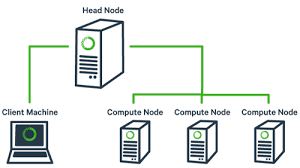
\includegraphics[width=0.65\columnwidth]{cluster}
	\caption{Rappresentazione di un cluster Hadoop (Fonte: \href{https://goo.gl/DgYJ4J}{https://goo.gl/DgYJ4J})}
\end{figure}

Il secondo obiettivo era lo studio dei tool principali che il team \textit{big data} utilizza per l'analisi ed il \textit{processing} dei dati, ovvero Hive, Impala, Spark. Oltre a questi tool di cui si è già dato un breve commento, l'azienda richiedeva lo studio di:
\begin{itemize}
	\item \textbf{Hue}\footcite{site:hue}: un'applicazione che offre un'interfaccia e semplifica alcune operazioni, come le \textit{query} su Hadoop, di cui è utile la conoscenza di base ma scarsamente utilizzato in quanto risulta relativamente complesso per utilizzi semplici;
	\item \textbf{Cloudera Manager}\footcite{site:cloudera}: una web app per la gestione dei servizi e dei tool di Hadoop. Permette di tenere sotto controllo il cluster, quindi le risorse disponibili e gli utenti collegati, e permette di gestire e visualizzare le attività dei tool attualmente in esecuzione e passati. È utilizzato principalmente dai \textit{system administrators} ma si rivela utile anche per il team \textit{big data} per un'analisi veloce del funzionamento \textit{real time} del sistema.
\end{itemize} 
\begin{figure}[!h] 
	\centering 
	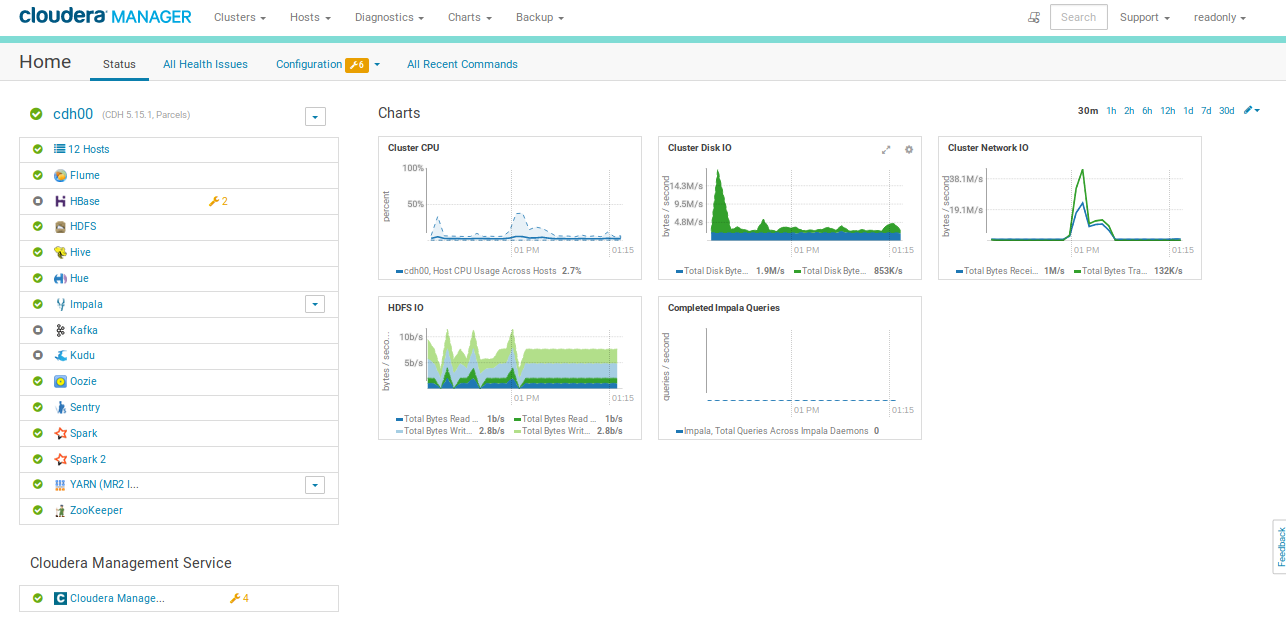
\includegraphics[width=1\columnwidth]{cloudera-manager}
	\caption{Interfaccia di Cloudera Manager}
\end{figure}
Al termine dello studio di questi tool, l'azienda richiedeva la comprensione e la successiva analisi del \textit{dataset} oggetto del progetto, che viene trattata in dettaglio nel capitolo successivo.
\subsection{Realizzazione di una web app per la presentazione dei risultati}
Dopo aver ottenuto tutti i dati di interesse, l'azienda richiedeva lo sviluppo di una \gls{web app} per la presentazione dei risultati in maniera più comprensibile ed appetibile rispetto a tabelle \gls{CSV} grezze. Grazie all'utilizzo di grafici, anche semplici, è infatti possibile notare alcune caratteristiche del \textit{dataset} che potrebbero rivelarsi utili ad una successiva analisi per la creazione del modello statistico.
%**************************************************************
\section{Vincoli}
\subsection{Vincoli metodologici}
Insieme con l'azienda, abbiamo deciso che avrei dovuto svolgere le attività di stage presso la sede della società. Questo è stato concordato con lo scopo di favorire il dialogo tra me ed il tutor aziendale e di avere la possibilità di confrontarmi direttamente con programmatori ed analisti più esperti in caso di problematiche durante lo svolgimento delle attività di progettazione, analisi e sviluppo software.
Oltre a ciò, l’azienda richiedeva che, al termine di ogni settimana lavorativa, venisse compilato un rapporto sulle attività che avevo svolto durante tale settimana. Inoltre, nel corso del primo periodo, prettamente di formazione, l'azienda richiedeva un breve resoconto di quanto compreso, cosicchè, in caso di dubbi, potessi confrontarmi con personale esperto prima di passare alla progettazione.
In seguito ad ogni rapporto, ed in particolare agli avanzamenti ed ai problemi incontrati descritti in esso, il tutor avrebbe deciso cosa avrei dovuto svolgere la settimana successiva, così da poter adattare al meglio il progetto al periodo di stage rimanente.\\
Al termine di tutte le attività, l'azienda richiedeva inoltre una breve presentazione di quanto svolto ad alcuni membri del management. Tale presentazione, esposta in forma verbale, mi sarebbe servita per illustrare ciò che avevo concluso tramite il progetto, elencando pro e contro della soluzione trovata.
\subsection{Vincoli temporali} \label{pdl}
Lo svolgimento dello stage prevedeva una durata di 320 ore complessive di lavoro. Queste ore sono state distribuite in modo uniforme in otto settimane lavorative da 40 ore ciascuna. Assieme al tutor aziendale, abbiamo concordato che l'orario di lavoro sarebbe stato dal Lunedì al Venerdì dalle 09:00 alle 18:00 con un'ora di pausa pranzo. Prima dell'inizio dello stage il tutor ha redatto nel Piano di Lavoro una scansione temporale delle attività su base settimanale.
In alcune occasioni, ho portato a termine il lavoro assegnato in anticipo, per cui abbiamo scelto di effettuare alcuni approfondimenti su argomenti che mi interessavano maggiormente, tramite lo studio autonomo ma con la possibilità di richiedere chiarimenti al personale più esperto che mi seguiva.
Il tutor ha quindi ripartito il lavoro su base settimanale nel seguente modo:
\begin{itemize}
	\item \textbf{Prima settimana}: 
		\subitem - consolidamento utilizzo sistema Unix;
		\subitem - comprensione mondo \textit{big data};
		\subitem - Apache Hadoop Architecture e \gls{HDFS}.
	\item \textbf{Seconda settimana}:
		\subitem - approfondimenti mondo \textit{big data};
		\subitem - apprendimento comandi \gls{HDFS};
		\subitem - comprensione tools Cloudera.
	\item \textbf{Terza settimana}:
		\subitem - approfondimento tools Cloudera;
		\subitem - studio ed esercitazione di Cloudera Impala ed Apache Hive.
	\item \textbf{Quarta settimana}:
		\subitem - studio ed esercitazione di Apache Spark;
		\subitem - comprensione di Cloudera Manager.
	\item \textbf{Quinta e sesta settimana}:
	 	\subitem - ripasso Java con attenzione all'ambiente Java EE;
	 	\subitem - studio del linguaggio scelto per il \textit{front-end}.
	\item \textbf{Settima e ottava settimana}:
		\subitem - applicazione delle principali tecnologie apprese al progetto.
\end{itemize}
Da questa suddivisione deriva il seguente \gls{Diagramma di Gantt}.
\begin{figure}[!h] 
	\centering 
	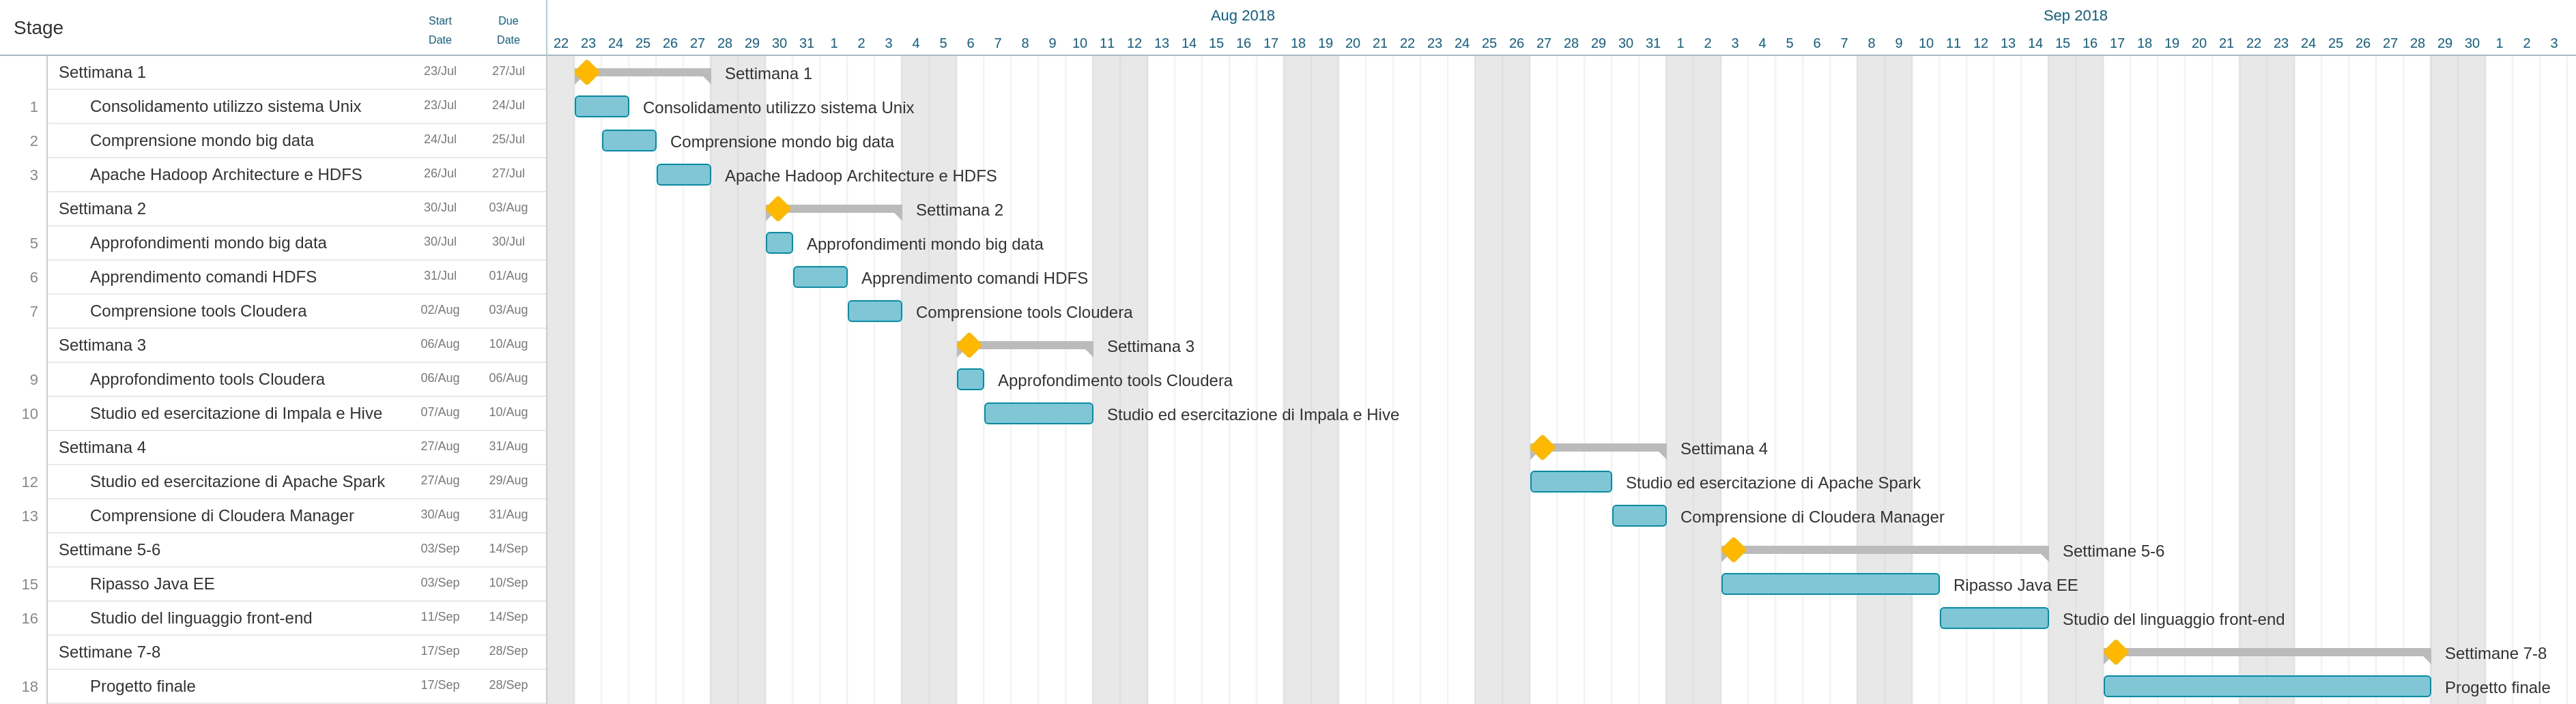
\includegraphics[width=1\columnwidth]{gantt}
	\caption{Diagramma di Gantt dello stage}
\end{figure}

\subsection{Vincoli tecnologici}
L'azienda, ad inizio stage, ha posto un unico vincolo per il progetto finale: utilizzare Java EE per la parte di \textit{back-end} del prodotto. Per la parte di \textit{front-end}, il tutor mi ha invece suggerito l'utilizzo di Angular, in quanto già assiduamente testato ed utilizzato per altri progetti, ma senza porre alcun tipo di vincolo, infatti la scelta finale dipendeva dalle mie preferenze ed esperienze passate. Inizialmente ho proposto come alternativa l'utilizzo delle librerie React\footcite{site:react} e Redux\footcite{site:redux} in quanto già in parte conosciute ed utilizzate. Come decisione finale però ho scelto, come proposto dall'azienda, Angular, in  quanto mi interessava come tecnologia e, vista la natura esplorativa di nuove tecnologie e strumenti dello stage, l'ho considerata la scelta migliore per il mio accrescimento culturale. \\
Per quanto riguarda la parte di \textit{big data}, mi sono affidato completamente al mio tutor aziendale, in quanto non avevo alcuna esperienza in quel campo e quindi non avrei potuto scegliere cosa fosse la scelta migliore per me. Oltre a ciò, gli strumenti utilizzati assieme ad Hadoop sono ormai consolidati e non c'è una grande varietà, quindi la scelta proposta dal personale aziendale si è rivelata obbligatoria. \\
Oltre a ciò, ho avuto la possibilità di utilizzare \gls{Git} per il versionamento del codice, che ho ben apprezzato ed utilizzato.
%**************************************************************

% DA RIVEDERE COME MAIL PRIMA DI INVIARE CAP3
\section{Aspettative personali sul progetto di stage}
Successivamente al mio impegno con l'azienda ed alla stesura del Piano di Lavoro, assieme alla definizione degli obiettivi, la mia curiosità verso l'argomento di stage si è intensificata. \\
Le aspettative che maggiormente sentivo erano:
\begin{itemize}
	\item Mettersi in gioco in un'azienda con partner di un certo livello nel mio campo di studi;
	\item Instaurare con il personale discussioni su esperienze e punti di vista diversi sulle varie tecnologie;
	\item Entrare in contatto con tecnologie nuove e sempre più di largo utilizzo;
	\item Conoscere il funzionamento di uno strumento come Hadoop e tutti i tool inerenti;
	\item Apprendere come effettuare un'analisi su un insieme di dati distribuiti in un \gls{cluster};
	\item Imparare come progettare e quali sono le \textit{best practice} per realizzare una \gls{web app} utilizzando Java EE.
\end{itemize}